\section*{Quickies 6}
\addcontentsline{toc}{subsection}{Quickies 6}

\subsection*{Angabe}
%\input{include/kompalg_angabe31}
/* \TeX sourcen fehlen */

%%%
% Lösung
%%%
\subsection*{Lösung}
\begin{flushenum}
%1.a
\item
\begin{flushalpha}
	\item Die Steigung der Strecke ist positiv und o.B.d.A. $> 1$ (für Steigung $<1$ erhält man das gleiche Ergebnis durch Spiegelung).
	\begin{figure}[h!]
		\begin{center}
		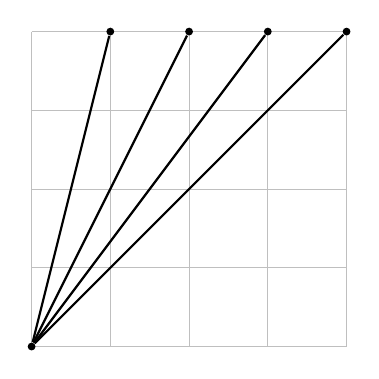
\begin{tikzpicture}
			\draw[step=1cm,color=lightgray] (0,0) grid (4,4);
			\node[fill,circle,inner sep=1pt] (o) at (0,0) {};
			\node[fill,circle,inner sep=1pt] (a) at (2,4) {};
			\node[fill,circle,inner sep=1pt] (b) at (3,4) {};
			\node[fill,circle,inner sep=1pt] (c) at (4,4) {};
			\node[fill,circle,inner sep=1pt] (d) at (1,4) {};
			\path (o) edge[thick] (a);
			\path (o) edge[thick] (b);
			\path (o) edge[thick] (c);
			\path (o) edge[thick] (d);
		\end{tikzpicture}
		\end{center}
	\end{figure}
	Wie in der Abbildung zu sehen ist, kann man grob zwei Fälle unterscheiden: Es werden Eckpunkte berührt oder es werden keine Eckpunkte berührt.
	Werden keine Eckpunkte berührt, werden offensichtlich pro Spalte $\lceil m \rceil$ Quadrate durchquert, bei Steigung $m$.
	Werden Eckpunkte berührt, kann man die Strecke auf das gleiche Problem reduzieren mit dem Rechteck der Größe $a/c \times b/c$,
	wobei $c = \gcd(a,b)$ ist und erhält so den Fall dass keine Eckpunkte berührt werden, da nun $a/c$ und $b/c$ teilerfremd sind.

	%1.b
	\item Man erreicht $t$ von $s$ aus gehend, wenn $a \mid \gcd(s,t)$. Man benötigt (mindestens) $\frac{|t-s|}{a}$ Schritte.

	%1.c
	\item Es muss gelten $s + x\cdot a + y \cdot b = t$, also muss $x\cdot a + y\cdot b = t-s$ gelten,
	und damit gilt $x'\cdot a + y' \cdot b = \gcd(s,t)$. Dies
	löst man mittels EEA. Man benötigt (mindestens) $x+y$ Schritte.
\end{flushalpha}

%2.a
\item 
\begin{flushalpha}
\item Per Induktion:
\begin{itemize}
	\item \textit{I.A.}: $n=0$: $x^0 - y^0 = 0$, $x-y \mid 0$ \\ $n=1$: $x-y \mid x^1 - y^1$ gilt offensichtlich.
	\item \textit{I.V.}: $\exists n \in \mathbb{N}$: $x-y \mid x^n - y^n$
	\item \textit{I.S.}: $n \rightarrow n+2$:
	\[ x-y \mid (x-y)(x^{n+1} + y^{n+1}) = x^{n+2} - y^{n+2} + x\cdot y^{n+1} - y \cdot x^{n+1} =\]
	\[ = x^{n+2} - y^{n+2} - xy \underbrace{(x^{n} - y^{n})}_{I.V.}\]
	Der rechte Teil des Ausdrucks ist nach \textit{I.V.} durch $x-y$ teilbar, da der ganze Ausdruck durch $x-y$ teilbar ist, muss dies auch $x^n - y^n$ sein.
\end{itemize}
Alternativer Beweis mit der geometrischen Reihe:
\[ \sum_{i=0}^{n-1}\left(\frac{y}{x}\right)^i = \frac{1-\left(\frac{y}{x}\right)^n}{1-\frac{y}{x}} \quad \vert \cdot x^{n-1}\]
\[ \Leftrightarrow x^{n-1}  \sum_{i=0}^{n-1}\left(\frac{y}{x}\right)^i = \sum_{i=0}^{n-1} y^ix^{n-1-i} = \frac{x^n}{x}  \frac{1-\left(\frac{y}{x}\right)^n}{1-\frac{y}{x}}  = \frac{x^n - y^n}{x-y} \]
Die linke Seite (Summendarstellung) ist eine ganze Zahl, da $y^i$ und $x^{n-1-i}$ für alle $i \in \{1, \ldots n-1\}$ ganze Zahlen sind. Also muss
die rechte Seite auch eine ganze Zahl sein, also gilt die gewünschte Teilbarkeitsbeziehung.

%2.b
\item Für $q=0$ ist das offensichtlich. Sei nun $q>0$. Dann gilt mit sukzessivem Ausklammern von $(n^b - 1)$:
\[
  n^a - 1 = n^{b\cdotq + r} - 1 = (n^b - 1)n^{b(q-1) + r} + n^{b(q-1) + r}-1 =
\]
\[
  = (n^b - 1)n^{b(q-1) + r} + (n^b - 1)n^{b(q-2) + r} + n^{b(q-2) + r} + \ldots
  +n^{b(q-q) + r} - 1 =\]\[= k \cdot (n^b-1) + n^r - 1
\]
Der Faktor $k$ ist somit \[ k = (n^a-1) \text{div} (n^b -1) = \sum_{i=1}^{q-1} n^{b\cdot i + r} \]
%2.c
\item Es gilt $\gcd(a,b) = \gcd(b,r)$ und $\gcd(n^a-1,n^b-1) = \gcd(n^b-1,n^r-1)$ nach voriger Teilaufgabe.
Da $gcd(a,b) = \ldots = gcd( gcd(a,b), 0)$ im letzten Schritt des Euklidischen Algorithmus gilt, ist somit $\gcd(n^a -1,n^b-1) = n^{\gcd(a,b)}-1$.
\end{flushalpha}
%3.
\item Der Zusammenhang zwischen $\gcd(a,b)$ und $\text{lcm}(a,b)$ ist: $\gcd(a,b) \cdot \text{lcm}(a,b) = |a \cdot b|$. Mit einem effizienten Algorithmus für $\gcd$ (Euklid)
hat man somit automatisch auch einen für $\text{lcm}$.

%4.
\item $\gcd(F_n, F_{n+1}) = \gcd(F_n, F_n + F_{n-1}) = \gcd(F_{n-1}, F_n) = \ldots = \gcd(F_0, F_1) = 1$
%5.
\item Mittels EEA kann man die Bézout-Koeffizienten bestimmen:
\[ s \cdot 17 \pm t \cdot 11 = \gcd(17,11) \]
Sowie Koeffizienten $a,b \neq 0$:
\[ a \cdot 17 \pm b \cdot 11 = 0 \]
Wenn $k \cdot \gcd(17,11) = 542$ gilt, hat man die Lösungsmenge:
\[ (s + i\cdot a)17 \pm (t + i\cdot b)11 = 542 \]
Die konkreten Zahlenwerte lassen dann erkennen wie groß die Lösungsmenge in $\mathbb{Z}$ bzw. $\mathbb{N}$ ist.

%6.
\item Lösung mittels EEA, Bézout-Koeffizienten. $s \cdot 15 + t \cdot 27 = \gcd(15,27) \mid  B$, $s,t \geq 0$ damit eine Lösung möglich ist.

%7.
\item $13 \equiv 2$ in $\mathbb{Z}_{11}$. EEA führt zum Ziel, Bézout-Koeffizienten modulo $11$ betrachten.

%8.
\item EEA für $\gcd(17,101)$ durchführen, der Bézoutkoeffizient der $17$ ist die Lösung.

%9.
\item EEA für $12$ und $236$, Bézout-Koeffizienten. Gilt $\gcd(236,12) \mid 30$, gibt es eine Lösung.

%10.
\item $\phi(46) = \phi(2) \cdot \phi(23) = 22$ ($\phi(p) = p-1$, $p$ prim).
 Inverse von $13$ und $31$ mittels EEA für $\gcd(13,46)$ bzw. $\gcd(31,46)$ durchführen, der entsprechende Bézout-Koeffizient ist das Inverse.
 Es gilt für alle $a$: $\text{ord}_{N} a \mid \phi(N)$ in $\mathbb{Z}_N^{\times}$. Damit ist die Ordnung von $a$ und $b$ entweder $11$ oder $22$.
 Berechnung von $3^{11} \equiv 1 \bmod 46$, also Ordnung $11$. $5^{11} \equiv 45 \equiv -1 \bmod 46$, also Ordnung $22$.

% 11.
\item Es gilt in $\mathbb{Z}_N^{\times}$: $a^x \equiv a^{x \bmod \phi(N)} \equiv a^{x \bmod \text{ord}_N a} \bmod N$.

% 12.
\item Es gilt $n = p\cdot q$, $q = n/p$, $\phi(n) = (p-1)(q-1) = p\cdot q - p - q + 1$. $n - \phi(n) = p + n/p - 1$. Dies ist eine quadratische Gleichung in p.

\end{flushenum}
